\documentclass{beamer}
\usetheme[
    sectionpage=progressbar
]{metropolis}             % Use metropolis theme
\setsansfont[	 	  % Fix needed to make fonts work: https://github.com/matze/mtheme/issues/280
	Extension      = .otf,
    UprightFont    = *-Light,
    ItalicFont     = *-LightItalic,
    BoldFont       = *-Regular,
    BoldItalicFont = *-RegularItalic
]{FiraSans}
\setmonofont[
    Extension   = .otf,
    UprightFont = *-Regular,
    BoldFont    = *-Medium
]{FiraMono}

\usepackage[german]{babel}

\definecolor{cioDarkBlue}{HTML}{12254c}
\setbeamercolor{normal text}{%
    fg=cioDarkBlue,
    bg=black!2
}

\graphicspath{ {img/} }

\title{Was sind Linux Container und wie funktionieren sie?}
\date{\today}
\author{Anian Ziegler}
\institute{cioplenu}

\begin{document}

  \maketitle
  \section{Was ist ein Container?}
  \begin{frame}{Was sind Container?}
    \begin{itemize}[<+->]
      \item \alert<4>{Virtualisierung auf Betriebssystemebene}
      \item Basiert auf meheren Features des Linux Kernels
      \item Isoliert und verpackt Anwendungen
    \end{itemize}
  \end{frame}
  
  \begin{frame}{Exkurs: Hardware-Virtualisierung}
    \includegraphics[width=\textwidth]{hypervisor}
  \end{frame}
  \begin{frame}{Exkurs: Hardware-Virtualisierung}
    \includegraphics[width=\textwidth]{vms}
  \end{frame}
  
  \begin{frame}{Virtualisierung auf Betriebssystemebene}
    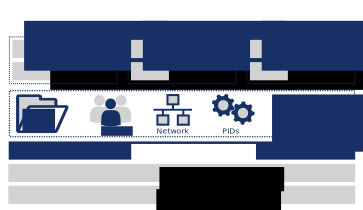
\includegraphics[width=\textwidth]{os-virt}
  \end{frame}
  \begin{frame}{Virtualisierung auf Betriebssystemebene}
  	\includegraphics[width=\textwidth]{container}
  \end{frame}
  \begin{frame}[standout]
    Demo
  \end{frame}

  \section{Implementierung in Linux}
  \begin{frame}{chroot}
    
\includegraphics[width=\textwidth]{fs-tree}
  \end{frame}
  \begin{frame}{chroot}
    \includegraphics[width=\textwidth]{fs-tree-highlight}
  \end{frame}
  \begin{frame}[standout]
    Demo
  \end{frame}
  \begin{frame}{chroot}
    \begin{itemize}
      \item Erlaubt es das root Verzeichnis \texttt{/} neu zu setzen
      \item Ermöglicht verschiedene Versionen eines Tools auf einem System zu installieren
      \item Sehr Hilfreich zum debugging oder bei der Installation von Linux
      \item \textbf{Aber:} Noch keine Isolierung der Prozesse, User etc. von einander
    \end{itemize}
  \end{frame}
  
  \begin{frame}{Namespaces}
    \begin{itemize}[<+->]
      \item API des Linux Kernel um \textbf{virtuelle System Ressourcen} wie Netzwerk Interfaces, Mount points, UserIDs und weitere System Ressourcen zu erstellen
      \item Diese Ressourcen können einzelnen Prozessen zugewiesen
werden
      \item Können auch für sich genommen verwendet werden: Auf seinem eigenen Rechner mit Network-Namespaces ein Netzwerk zu simulieren
    \end{itemize}
  \end{frame}
  
  \begin{frame}{Control Groups}
    \begin{itemize}[<+->]
      \item Management von CPU Zyklen, Arbeitsspeicher oder Netzwerk Bandbreite für Gruppen von Prozessen
      \item Prozesse können in ihrem Ressourcenverbrauch eingeschränkt werden
      \item Auch seperat Nutzbar
    \end{itemize}
  \end{frame}
  
  \section{Vergleich mit VMs}
  \begin{frame}{Vergleich mit VMs}
    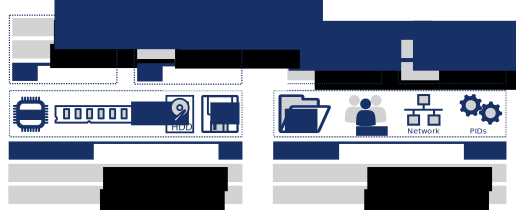
\includegraphics[width=\textwidth]{comparison}
    \textbf{Unterschied:} Bei VMs wird im Kernel/Hypervisor Hardware virtualisiert und darauf laufen andere Kernels. Container teilen sich einen Kernel, der OS-Ressourcen virtualisiert. 
  \end{frame}
  \begin{frame}{Vorteile VMs}
    \begin{itemize}
      \item Voller virtueller Computer mit allen Features
      \item Egal welcher Kernel: Linux, BSD, Windows NT, x86, x64
      \item Starke Isolierung
    \end{itemize}
  \end{frame}
  \begin{frame}{Vorteile Container}
    \begin{itemize}
      \item Effizienter: Weniger Ressourcenverbrauch und kein Boot-Vorgang
      \item Einfacher zu managen
      \item Auch einzelne Module verwendbar
    \end{itemize}
  \end{frame}
  
  \section{Praktische Anwendung}
   
  \section{Geschichte}
  \begin{frame}{Was sind Container?}
    Hello, Hackerkiste!
  \end{frame}


  \begin{frame}[standout]
    Fragen?
  \end{frame}
\end{document}

